\section{Unit-tests}
At Unitteste er at teste enkelte moduler i koden. Vi tester vores kode for at fange eventuelle bugs og mangler på et tidligt stadie. Når man skriver sine tests, tvinges man samtidig til at tænke mere over det stykke kode man har skrevet.

\subsection{Terminologi}
\begin{itemize}
	\item Unit test - Et stykke kode, typisk en metode, der bruger et andet stykke kode for at teste nogen antagelsers korrekthed.
	\item Unit - En metode.
	\item System Under Test - Det system man tester på.
\end{itemize}

\subsection{En god Unittest}
\begin{itemize}
	\item Automatiseret og repeatable.
	\item kan ogaå bruges i morgen.
	\item Skal kunne køres blot ved hjælp af et tryk på en knap.
	\item Skal køre hurtigt.
	\item Skal producere samme resultat hver gang.
	\item Skal køre isoleret fra andre tests.
	\item Ved fejl skal det tydeligt fremgå hvad der er galt.
\end{itemize}

\subsection{Hvordan Unittester vi?}

Vi bruger testframeworket NUnit. NUnit giver bla. mulighed for:

\begin{itemize}
	\item Detaljerede fejlrapporter - Beskriver hvorfor en test fejler.
	\item Setup og teardown, se figur~\ref{fig:testFixture}
	\item At nemt indsætte nye tests i systemet.
\end{itemize}

\subsubsection{NUnit attributter}

\paragraph{[TestFixture]} Indikerer en klasse der indeholder automatiserede NUnit tests. 
\paragraph{[Test]} Indikerer en enkelt automatiseret test.
\paragraph{[TestCase]} Indikerer en test med parametre.
\paragraph{[SetUp]} Indikerer en SetUp metode. Køres hver gang en test i samme TestFixture køres.
\paragraph{[TearDown]} Indikerer en TearDown metode. Køres hver gang en test i samme TestFixture er afsluttet. Bruges til at nulstille.

\subsubsection{Naming conventions}
Der er nogle konventioner man følger når testmetoder skal navngives, demonstreret i Code listing~\ref{code:namingconvention}.

\begin{lstlisting}[caption=Eksempel på navngivnings konvention for test.,label=code:namingconvention]
[Test]
public void NameOfMethod_FunctionalityToBetested_ExpectedOutcome()
{
	// assert something here...
}
\end{lstlisting}

Når der skrives en Unittest, følger man typisk de tre A'er.

\begin{itemize}
	\item Arrange - Instantiering af UUT objekt.
	\item Act - Stimuler UUT til at gøre det vi ønsker - \textit{result = UUT.someMethod()}.
	\item Assert - Assertion på om vi får det forventede resultat. \textit{Assert.False(result)}.
\end{itemize}

\subsubsection{Parametiserede tests}
I NUnit er der mulighed for at at bruge parametiserede tests. Dette er nyttigt hvis man ønsker at køre samme test med flere forskellige parametre. I stedet for at bruge \textbf{Test} attributten, bruges \textbf{TestCase(param1, param2)} attrbutten.

\begin{figure}[H]
\centering
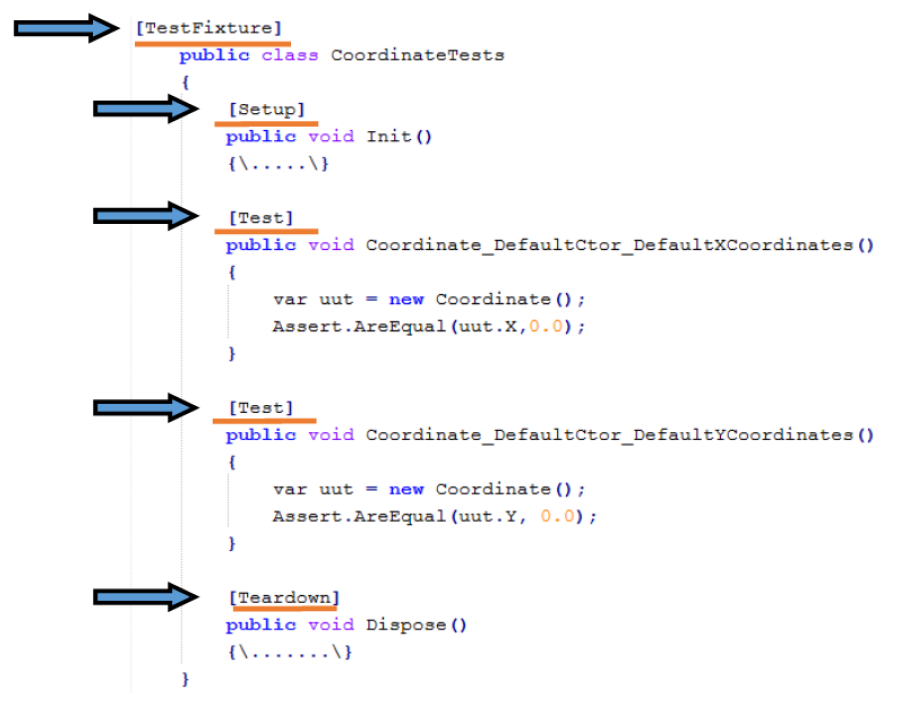
\includegraphics[width=0.7\linewidth]{figs/testFixture.PNG}
\caption{Syntaks for unittesting i NUnit}
\label{fig:testFixture}
\end{figure}

\subsection{Assertion models}
Der findes to typiske måder at asserte på. Den ene kaldes den klassiske model og den anden kaldes Constraint baseret.

Den klassiske assert anvender AreEqual metoden. Denne tager to parametre, en værdi samt metoden som ønskes testet - her om den returnerer den korrekte værdi.
\begin{figure}
\centering
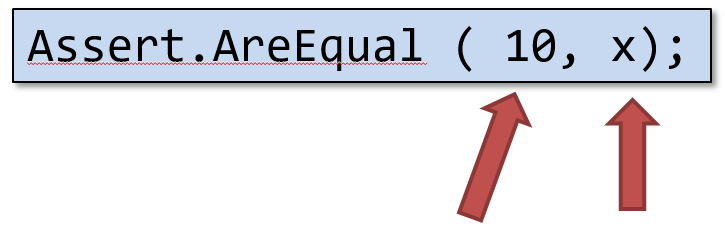
\includegraphics[width=0.7\linewidth]{figs/classicAssert.PNG}
\caption{Classic Assert model}
\label{fig:classicAssert}
\end{figure}


